\documentclass[letterpaper,11pt]{article}
\usepackage{jheppub}

\begin{document}

%%%%%%%%%%%%%%%%%%%%%%
\section*{GAN-AE and BumpHunter}
Author(s): Louis VASLIN, Julien DONINI \\ \textit{Laboratoire de Physique de Clermont, Université Clermont Auvergne, France}\\


\subsection{Method}
\label{sec:method}

\noindent The methods presented in this paper combine two independent anomaly detection algorthm.
The objective is to have a full analysis workflow that can give a global p-value and evaluate the number of signal events in any black-box dataset.

\subsubsection{GAN-AE}
\label{sec:GAN-AE}

\noindent The GAN-AE method is an attempt at associating an Auto-Encoder architecture to a discriminant neural network in a GAN-like fashion.
The reason for this particular setting is to use information that does not come only from the "reconstruction error" usualy used to train AEs.
This could be seen as a alternative way to constrain the training of an AE.
As discriminant network, a simple feed-forward Multi-Layer Perceptron (MLP) is used. \\

\noindent This method been inspired by the GAN algorithm, the two participants (AE and MLP) are trained alternatively with opposite objectives :

\begin{itemize}
	\item The MLP is trained for a few epochs using the binary crossentropy (BC) loss function on a labeled mixture of original and reconstruted events, the objective being to expose the weaknesses of the AE.
	
	\item The AE is trained for a few epochs using a loss function combining the reconstruction error (here, the Mean Euclidean Distance between the input and output, or MED for short) and the BC loss of the MLP.
	In order to decorrelate as much as possible the reconstruction error and the invariant mass, the distance correlation (DisCo) term is used~\cite{DiscoFever}.
	The loss is then given by :
	$$loss_{AE} = BC+\varepsilon\times MED+\alpha\times DisCo$$
	\noindent With $\varepsilon$ and $\alpha$ two hyperparameters used to balance the weights of each terms. In this case, the BC term is evaluated by giving reconstructed events to the MLP, but this time with the "wrong label", the objective being to mislead the MLP. 
	
	\item Then the AE is evaluated on a validation set using a Figure of Merit (FoM) that also combines the reconstruction error and some information from the MLP.
	The FoM used is given by :
	$$FoM = MED+(1-Mean~MLP~output)$$
	\noindent This second term is preferred over the binary crossentropy because it seems to be more stable, which makes it more suitable to set a early stopping condition.
	As for the reconstruction error, $1-Mean~MLP~output$ must be minimized.
	In fact, the closer to zero is this term, the better the AE is at misleading the MLP.
\end{itemize}

\noindent These three steps are repeated in a loop until the FoM fails to improve for five cycles. Once the AE has been trained, the MLP can be discarded since it is not needed anymore. Then, the AE can be used by taking the reconstruction error (Euclidean distance) as discriminative feature.\\

\noindent For the LHC Olympics, the following hyerparameter were used ...

\subsubsection{BumpHunter}
\label{sec:BH}

\noindent The BumpHunter algorithm is a hypertest that compares a data distribution with a reference and evaluates the p-value and significance of any deviation.
To do so, BumpHunter will scan the two distributions with a sliding window of variable width.
For each position and width of the scan window, the local p-value is calculated. The window corresponding to the most significant deviations is then defined as the one with the smallest local p-value.\\

\noindent In order to deal with the look elsewhere effect and evaluate a global p-value, BumpHunter generates pseudo-experiment by sampling from the reference histogram.
The scan is then repeated for each pesudo-data histogram by comparing with the original reference.
This gives a local p-value distribution that can be compared with the local p-value obtained for the real data.
Thus, a global p-avlue and significance is obtained.
%In order to evaluate the number of signal events, the difference of event count in the bump window for the data and the reference can be used.

\noindent For the LHC Olympics, the following hyerparameter were used ...

\subsubsection{Full analysis workflow}

\noindent The objective of this work is to use the Auto-Encoder trained withe the GAN-AE algorithm to reduce the background and then use the BumpHunter algorithm to evaluate the (global) p-value of a potential signal.
However, the use of this second algorithm requires the use of a "reference background" to be expected in the data.
Unfortunately, such reference is not always available, as it is the case for the LHC Olympics black-box dataset.
Thus, in order to use BumpHunter, one must first extract a background model for the data.\\
Another point that has to be taken into acount is the fact that, despite the use of the DisCo term, the dijet mass spectum is not totally independent from the reconstuction error.
Thus, simply rescaling the full dataset precut to fit the mass spectrum postcut will not work. \\

\noindent One way to do this is to use a small subset of the data to compute a shaping function.
The objective of this function is to capture how the mass spectum behaves when a cut on the reconstruction error is applied.
This function is computed bin per bin on the dijet mass histogram by doing the ratio of the bin yields postcut and precut.\\
Of course, the presence of signal in the subset used for this calculation might impact this shaping function.
In order to mtigate this efect, the shaping function can be fitted using the tools available in the scikit-learn toolkit.
This will minimize the effect of the signal on the shaping function.\\
Once the shaping function is defined, it can be used to reshape the mass spectum precut in order to reproduce the behaviour of the background postcut.\\

\noindent With this final step, the full analysis workflow is the following :
\begin{itemize}
	\item Data preprocessing (anti-Kt clusturing, precut on dijet mass)
	\item Training of GAN-AE on the RnD background
	\item Application of the trained AE on the black-box dataset
	\item Use 100k events for the black-box to compute a shaping function
	\item Use the shaping function to build a reference to use the BumpHunter algorithm
\end{itemize}



\subsection{Results on LHC Olympics}
\label{sec:results}

\noindent The results shown were obtained with an AE trained with the GAN-AE algorithm on 100k events from the RnD bakground.
Note that before the training and application, cuts were applied on the dijet mass at 2700 GeV and 7000 GeV.


\subsubsection{R\&D dataset}
\label{sec:RnD}

\noindent Here we discuss the result obtained on the R\&D dataset.
The trained AE have been tested on 100k background events (not used during the training), as well as on the two signals provided.
On Fig.~\ref{fig:fig1} is shown the Euclidean distance distributions (left) and the corresponding ROC curves (right).\\

\noindent This result shows the potential of the GAN-AE algorithm to obtain a good discrimination between the background and signals, event though only the background was used during the training.
However, if the obtained AUC is good, it also appears that the Euclidean distance is still very correlated with the dijet mass.
This might have a negative impact on the bump hunting algorithm performance.

\subsubsection{Black-Boxes dataset}
\label{sec:BB}

\begin{figure}[h!]
\centering
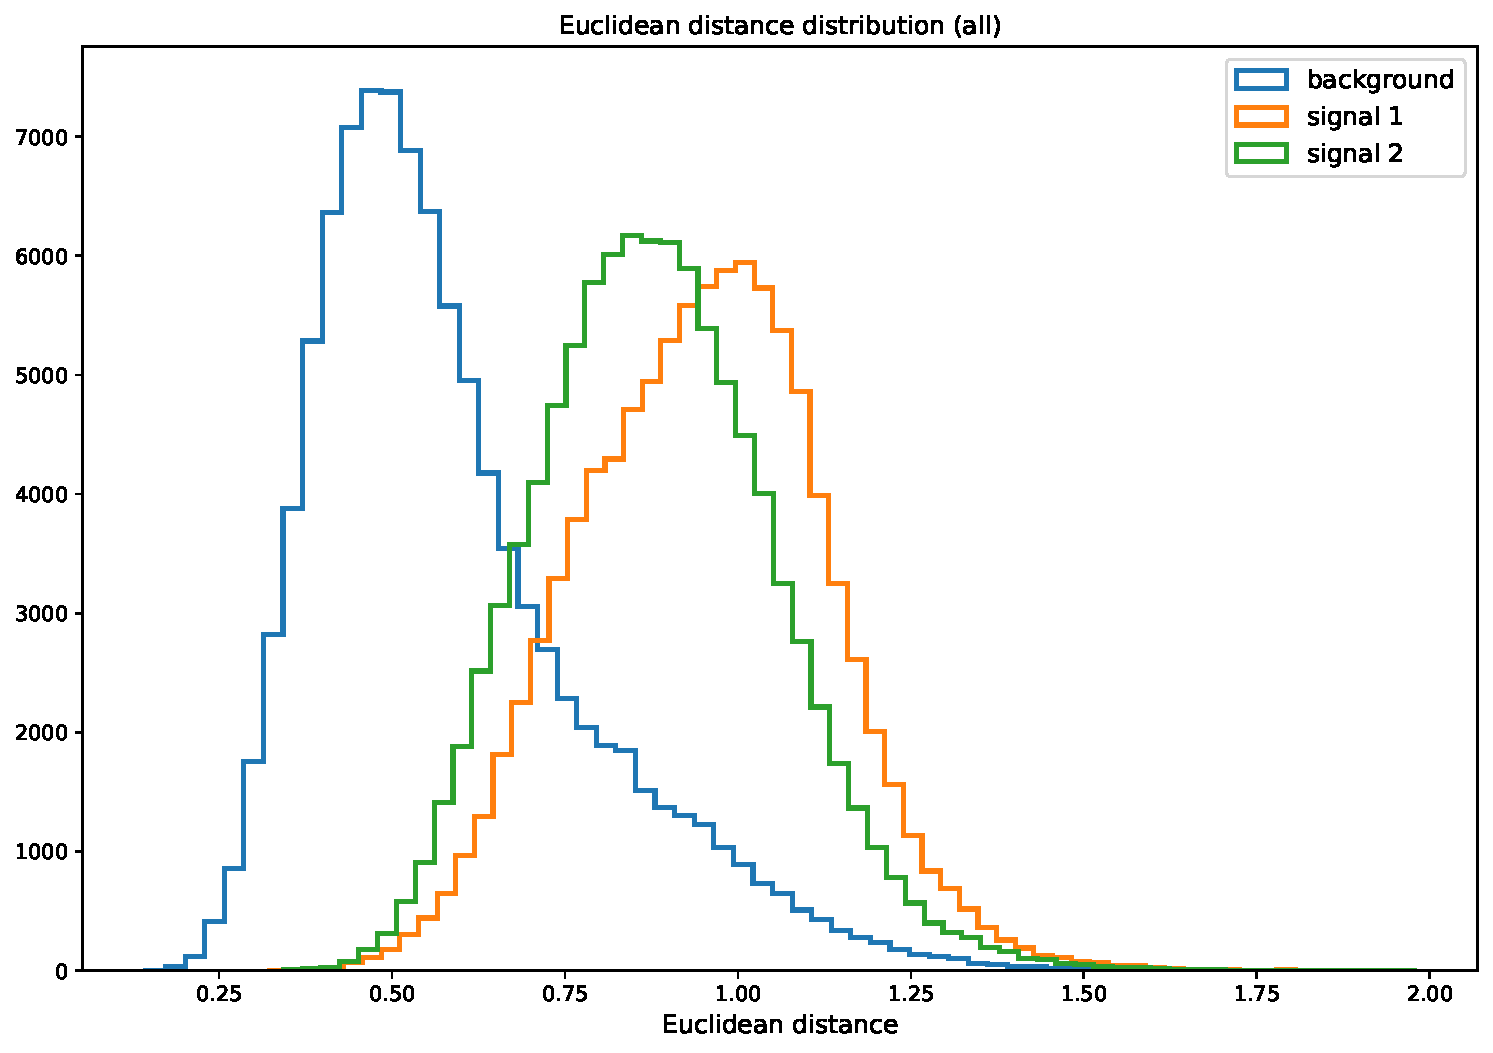
\includegraphics[width=0.49\textwidth]{img/RnD_single_distance_all.pdf}
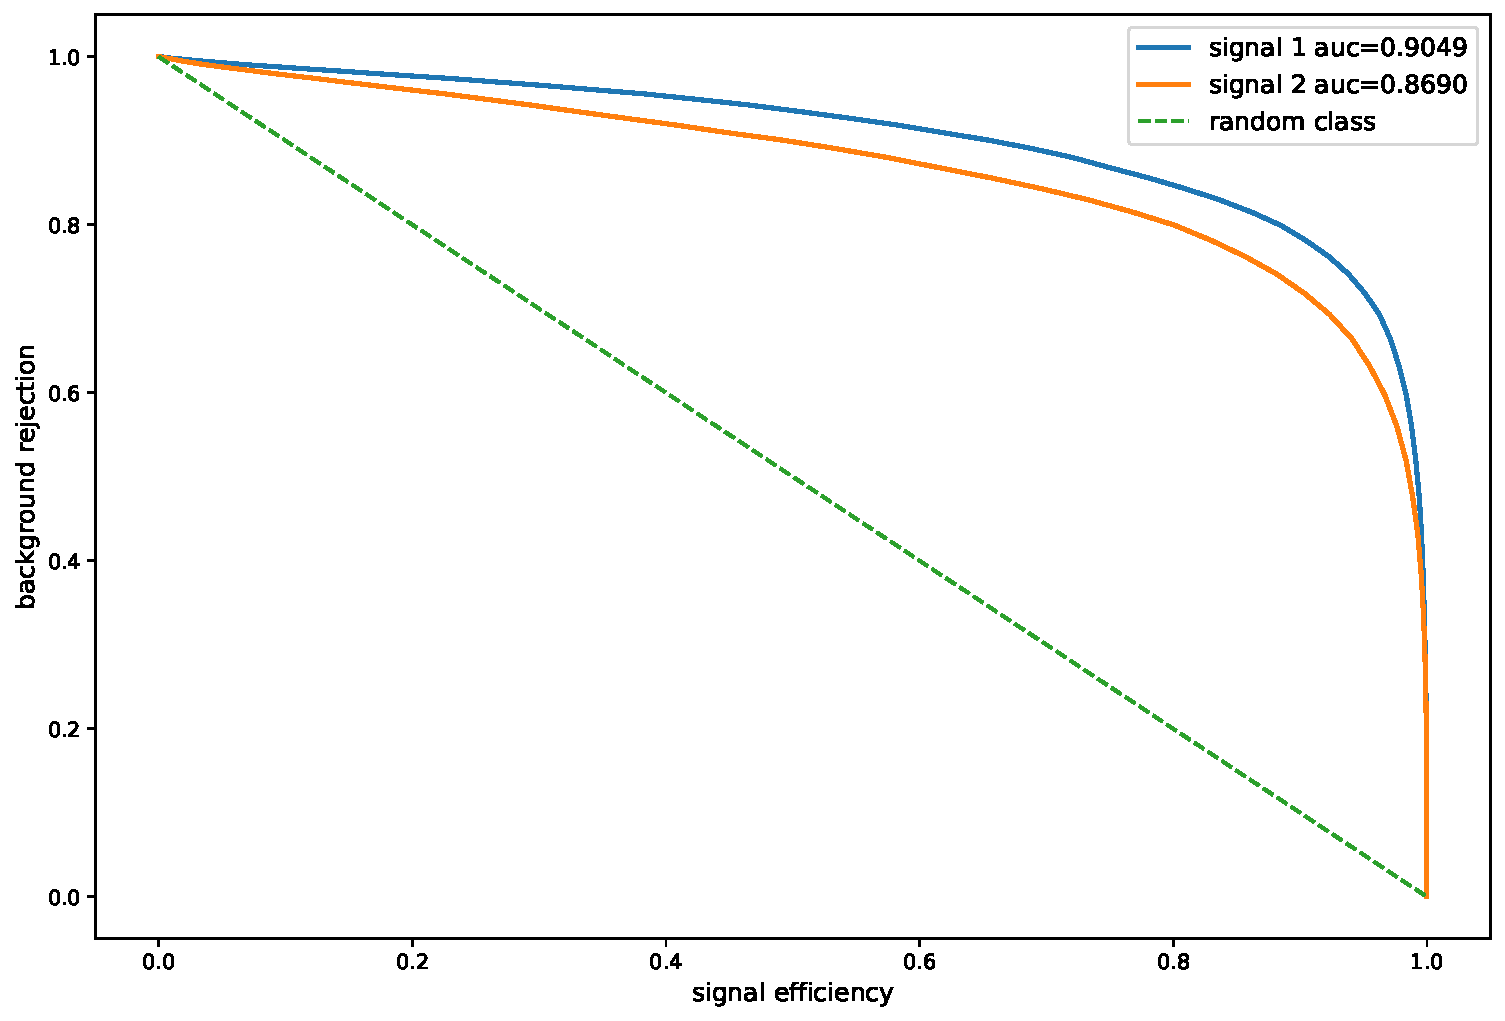
\includegraphics[width=0.49\textwidth]{img/RnD_single_ROC_all.pdf}
\caption{Euclidean distance distributions and ROC curves obtained for the R\&D dataset.}
\label{fig:fig1}
\end{figure}


\subsection{Lessons Learned}
\label{sec:lessons}

\noindent \textit{Please say anything that you learned from the experience in general, what you learned specifically from the results, what you improved after you learned about BB1, what you would change in the future, etc.}

\subsection{Code Availability}
\label{code:code}

\noindent All the scripts used to train and apply the GAN-AE algorithm are given at this link :\\

\noindent The implementation of the BumpHunter algorithm used in this work can be found at this link :\\
\href{https://github.com/lovaslin/pyBumpHunter}{https://github.com/lovaslin/pyBumpHunter}\\
\noindent In near future, it is planed that this implementation of BumpHunter becames a official package that might be added to the scikit-HEP toolkit.

%%%%%%%%%%%%%%%%%%%%%%%%
\acknowledgments

This work was supported by the U.S.~Department of Energy, Office of Science under contract DE-AC02-05CH11231. 

\vspace{10mm}

\noindent \textit{For the references, please use names from Ref.~\cite{hepmllivingreview}.  If your paper is not there or is not updated, please submit a MR!}

\bibliographystyle{jhep}
\bibliography{HEPML}
\end{document}
